\chapter{Testovacie API}

\label{kap:prakticke} % id kapitoly pre prikaz ref

V tejto kapitole navrhneme, implementujeme a otestujeme jednoduché rozhranie so schémou zabezpečenia využívajúcou jednotlivé tokeny popísané v kapitole \ref{kap:typy} a teoreticky porovnané v kapitole \ref{kap:teoreticke}. Nepriehľadný token budeme, na rozdiel od prechádzajúcej kapitoly, chápať iba ako náhodný reťazec. Cieľom implementácie je porovnať rýchlosť spracovania požiadaviek využívajúcich rôzne tokeny na autorizáciu a jednoduchosť práce s knižnicami implementujúcimi jednotlivé tokeny vo vybranom programovacom jazyku. Implementácia môže zároveň slúžiť ako základ pre implementovanie jednoduchej schémy zabezpečenia a jej integrovanie s vybranými knižnicami. Zdrojový kód je dostupný na platforme GitHub\footnote{Zdrojový kód je dostupný na adrese:\\ https://github.com/jitka1997/bachelor-thesis/tree/main/simpleAPI} a v prílohe A.

\section{Použité technológie}

Testovacie API sme implementovali v jazyku JavaScript, konkrétne pomocou prostredia Node.js. Použili sme knižnicu Express.js, ktorá umožňuje ľahko implementovať jednoduchý server.

Na vytváranie a validáciu jednotlivých tokenov sme použili knižnice pre JavaScript z~tabuľky \ref{tab:implementacie}, ktoré sme použili pri porovnaní popularity tokenov. Implementovali sme aj NONE token, reprezentujúci samotnú réžiu okolo vytvorenia a spracovania volania na API. Pre Biscuits neexistuje knižnica pre JavaScript, preto sme Biscuits v tejto kapitole neporovnávali. Prácu s~nepriehľadným tokenom sme implementovali sami. Informácie spojené s nepriehľadným tokenom si ukladáme v databáze. Využili sme jednoduchú databázu sqlite.

Klienta vykonávajúceho požiadavky na rozhranie sme tiež naprogramovali v Node.js.

Pre interpretáciu nameraných výsledkov sme použili jazyk Python a knižnice: numpy pre prácu s vektormi čísel, matplotlib pre generovanie grafov a jinja2 pre prácu s HTML šablónou.

\section{Popis rozhrania}

Vytvorili sme rozhranie s dvoma koncovými bodmi \textit{signin} a \textit{welcome}. Prvý z nich slúži na získanie tokenu klientom a druhý na vykonanie požiadavky, ktorá bude úspešná len v~prípade, že bude obsahovať platný token, ktorý rozhranie úspešne validuje. Na získanie tokenu sa klient musí úspešne autentifikovať pomocou základnej HTTP autentifikácie, teda zaslaním base64url \cite{base64_rfc} zakódovaného mena a hesla v autentifikačnej hlavičke požiadavky.

Rozhranie overí korektnosť prihlasovacích údajov a ak sú správne, tak vygeneruje token. V reálnom systéme by boli prihlasovacie údaje uložené v databáze, kde by ich rozhranie overilo. My pre jednoduchosť databázu používateľov simulujeme pomocou načítania objektu s používateľmi zo súboru usersDB. V tomto objekte sú používateľské mená a~heslá uložené ako dvojice kľúč a hodnota.

Po úspešnej autentifikácii vygeneruje rozhranie token a vráti ho klientovi. Klient následne môže token použiť na vykonanie požiadavky na koncový bod \textit{welcome}. Rozhranie overí platnosť tokenu a ak je platný, vykoná požiadavku, teda vráti klientovi uvítaciu správu obsahujúcu jeho prihlasovacie meno získané z tokenu. Ak token nebol zaslaný alebo zlyhá jeho validácia, rozhranie vráti klientovi chybový kód.

\section{Obsah a generovanie tokenu}
\label{sec:obsah}

Obsahovo vytvárame token nesúci štyri informácie overované pri autorizácii. Konkrétne čas vypršania platnosti tokenu, prihlasovacie meno používateľa, identifikátor vydavateľa tokenu a identifikátor prijímateľa tokenu. Čas vypršania platnosti tokenu je 5~minút od jeho vydania, identifikátory vydavateľa a prijímateľa sú pevne stanovené hodnoty a prihlasovacie meno je získané z prihlasovacích údajov klienta.

Tieto informácie sme do obsahu tokenu pridali, aby sme demonštrovali využitie údajov z tokenu na autorizáciu požiadavky, prípadne identifikáciu používateľa. Do konkrétneho tokenu sme vložili informácie spôsobom, ktorý nám umožnila špecifikácia daného tokenu a použitá knižnica implementujúca token. Konkrétne:


\begin{itemize}
    \item Nepriehľadný token -- do databázy sme vložili riadok obsahujúci samotný token ako identifikátor a ostatné informácie ako hodnoty jednotlivých stĺpcov.
    \item JWT a PASETO -- meno používateľa sme vložili do tela tokenu ako oprávnenie \textit{username} a ostatné informácie ako štandardné oprávnenia.
    \item Fernet -- všetky informácie sme vložili ako serializovaný JSON objekt do tela tokenu. Fernet síce obsahuje samostatnú časovú pečiatku, no vybraná knižnica nepodporuje jej použitie na validáciu časovej platnosti tokenu.
    \item Branca -- čas vypršania platnosti tokenu sme zaznamenali ako časovú pečiatku vytvorenia tokenu a následne pri jeho validácii sme určili ako stará môže táto časová pečiatka byť. Ostatné informácie sme vložili do tela tokenu ako serializovaný JSON objekt.
    \item Macaroons -- všetky informácie sme do tokenu vložili ako pravidlá prvej strany.
\end{itemize}

NONE token sme implementovali ako samotné prihlasovacie meno používateľa. Token sa nešifruje ani nepodpisuje a nemá ani žiadnu štruktúru. Ide len o reťazec reprezentujúci prihlasovacie meno používateľa.

JWT a PASETO, aj vybrané knižnice, ktoré ich implementujú, ponúkajú viacero funkcií na podpísanie a prípadné šifrovanie tokenu. Ostatné tokeny však používajú na podpisovanie jedinú funkciu, vždy variant hešovania s kľúčom. Fernet a Branca navyše šifrujú telo tokenu. Preto sme pre objektívne porovnanie tokenov zvolili pri JWT a~PASETO, čo najpodobnejšie funkcie na podpisovanie a taktiež šifrujeme telo tokenu. Šifrovacie funkcie sme tiež vybrali tak, aby boli najpodobnejšie šifrovacím funkciám v ostatných tokenoch. Kryptografické funkcie použité na podpisovanie a šifrovanie jednotlivých tokenov sú uvedené v tabuľke \ref{tab:funkcie}.

\begin{table}[H]
  \begin{center}
    \caption{Kryptografické funkcie na podpisovanie a šifrovanie tokenov}
    \label{tab:funkcie} % create a label for the table, after caption

    \resizebox{\columnwidth}{!}{%
    \begin{tabular}{lcccccc}
      \hline
      Proces & Nepriehľadný & JWT & PASETO & Fernet & Branca & Macaroons \\
      \hline
      Šifrovanie & $\varoslash$ & AES-128-CBC & AES-256-CTR & AES-128-CBC & XChaCha20 & $\varoslash$ \\
      Podpisovanie & $\varoslash$ & HMAC-SHA256 & HMAC-SHA384 & HMAC-SHA256 & Poly1305 & HMAC-SHA256 \\
      \hline
    \end{tabular}%
    }
  \end{center}
\end{table}

\section{Práca s knižnicami}

Pre každý token sme pomocou danej knižnice implementovali 2 funkcie -- \textit{createToken(username)} a \textit{verifyToken(token)}. Funkcia \textit{createToken} vráti nový token s obsahom a formátom popísaným v podkapitole \ref{sec:obsah}. Funkcia \textit{verifyToken} validuje podpis tokenu. Následne dešifruje telo tokenu (ak bolo zašifrované) a validuje jeho obsah. Ako kľuč pre kryptografické funkcie sme používali konštantný náhodne vygenerovaný reťazec s~potrebným počtom bitov.

Jednoduchosť práce s knižnicami implementujúcimi tokeny porovnávame na základe podpory jednoduchého generovania tokenu a štandardných validácií tela tokenu.
Všetky knižnice podporujú jednoduché podpísanie a prípadné šifrovanie tokenu. Takisto všetky knižnice podporujú validáciu podpisu tokenu. 

Pre JWT a PASETO nám knižnice ponúkli viacero štandardných oprávnení, ktoré sme mohli použiť pri vytváraní obsahu tokenu. Potom pri validácii tokenu stačilo uviesť požadované hodnoty týchto oprávnení a knižničné volanie ich validovalo. Fernet nepodporuje nijaké štandardné validovanie obsahu tokenu ani na úrovni špecifikácie, teda ani knižnica, ktorá ho implementuje, ho neponúkala. Overovanie formátu a obsahu tela tokenu sme teda implementovali sami. Branca podobne ako Fernet na úrovni špecifikácie neponúka štandardnú validáciu tela tokenu. No vybraná knižnica umožňuje validovať aspoň časovú platnosť tokenu pomocou časovej pečiatky v tokene a časového limitu zadaného ako argument pri dešifrovaní tela. Ani špecifikácia Macaroons nepodporuje žiadnu štandardnú validáciu pravidiel. Vybraná knižnica dovoľuje jednoducho pridávať pravidlá prvej strany tým, že riadi réžiu okolo postupného generovania podpisu tokenu. Neexistujú však žiadne štandardné pravidlá a preto sme ich validáciu implementovali sami.

NONE token slúži len na odmeranie času potrebného na réžiu spojenú s vykonávaním požiadaviek rozhraním, preto ho v tejto podkapitole neporovnávame.

Na základe týchto pozorovaní sme porovnali jednoduchosť práce s rôznymi tokenmi, rovnakým spôsobom ako vlastnosti porovnané v tabuľke \ref{tab:porovnanie} pomocou symbolov \CIRCLE, \LEFTcircle, \Circle ~a $\varoslash$. Výsledky sú uvedené v tabuľke \ref{tab:api_porovnanie}.

\begin{table}
  \begin{center}
    \caption{Jednoduchosť práce s knižnicami}
    \label{tab:api_porovnanie} % create a label for the table, after caption

    \resizebox{\columnwidth}{!}{%
    \begin{tabular}{lcccccc}
      \hline
      Vlastnosť & Nepriehľadný & JWT & PASETO & Fernet & Branca & Macaroons \\
      \hline
      Jednoduchosť práce & $\varoslash$ & \CIRCLE & \CIRCLE & \Circle & \Circle & \LEFTcircle
    \end{tabular}%
    }
  \end{center}
\end{table}

\section{Meranie rýchlosti}

Pre porovnanie rýchlosti spracovania požiadavky sme implementovali jednoduchého klienta vykonávajúceho požiadavky na rozhranie. Klient sa najprv úspešne autentifikuje voči rozhraniu, ktoré mu vráti platný prístupový token. Následne klient vytvorí požiadavku na rozhranie s týmto tokenom.

Klient teda vykonáva jednu požiadavku bez tokenu, na ktorej vykonanie musí rozhranie vygenerovať nový token a jednu požiadavku s platným tokenom, na ktorej vykonanie musí rozhranie validovať token. Teda v princípe meriame čas generovania a validácie tokenu. Na meranie času vytvorenia tokenu meria klient čas od odoslania požiadavky na autentifikáciu po vrátenie tokenu rozhraním. Na meranie času validácie tokenu meria klient čas od odoslania požiadavky na rozhranie po vrátenie odpovede rozhraním.

Pre presnejšie meranie meriame čas ako súčet 100 iterácií zaslania a spracovania požiadavky. Všetky namerané hodnoty sú teda súčtom 100 meraní a pre vyjadrenie času vykonania jednej požiadavky je nutné ich predeliť 100. Celý proces opakujeme 1000 krát. Klient teda vykoná spolu 100000 požiadaviek na autentifikáciu (generovanie tokenu) a 100000 požiadaviek s tokenom (validácia tokenu). Výsledky merania, ktoré používame na analýzu rýchlosti tokenov sú zaznamenané v súbore used\_measurements v elektronickej prílohe a v zdrojovom kóde na platforme GitHub.

\section{Analýza nameraných výsledkov}
\label{sec:vyhodnotenie}

V tejto podkapitole uvedieme a popíšeme vybrané grafy, ktoré sme vygenerovali z nameraných hodnôt. Z každého grafu uvedieme dva varianty. Prvý vypočítaný z meraní generovania tokenu a druhý z meraní validácie tokenu. Keď budeme hovoriť o rýchlosti tokenu, myslíme tým rýchlosť generovania a validácie daného tokenu.

Vhodný graf pre vizualizáciu rozloženia dát je krabicový graf. Na grafe vidíme krabicu, ktorej hornú a dolnú hranu tvoria 1. a 3. kvartil. Vnútri krabice je plnou čiarou znázornený medián (2. kvartil) a čiarkovanou čiarou je znázornený aritmetický priemer. Z krabice vystupujú do dvoch strán takzvané fúzy. Hranice fúzov reprezentujú poslednú hodnotu v rámci 1,5 násobku medzikvartilového rozpätia. Medzikvartilovým rozpätím rozumieme rozdiel medzi 3. a 1. kvartilom. Všetky hodnoty, ktoré sú väčšie ako hranica horného fúzu alebo menšie ako hranica dolného fúzu sú považované za odľahlé hodnoty a sú znázornené malými kružnicami. V našom prípade zobrazuje ľavá os čas v milisekundách.

\begin{figure}[H]
  %vlozenie samotneho obrazku vycentrovaneho a vhodnej velkosti
  %obrazok je v subore images/session.png
  \centerline{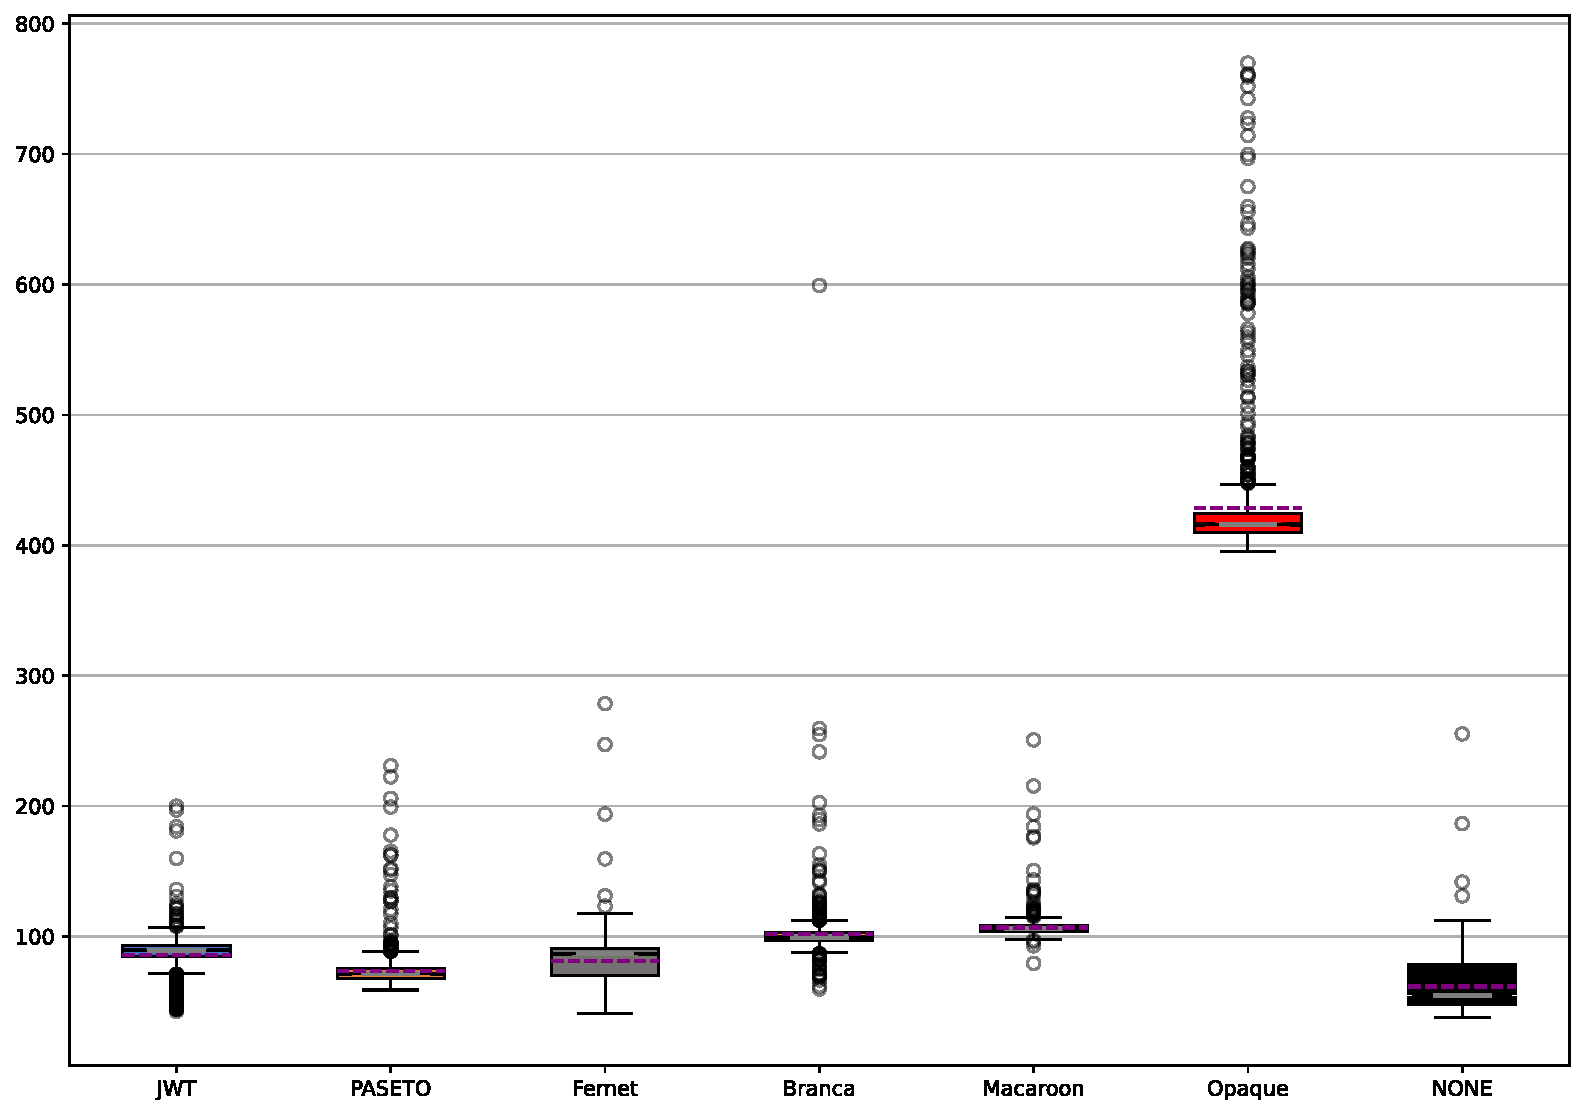
\includegraphics[width=0.7\textwidth]{images/signin_boxplot_allW}}
  %popis obrazku
  \caption[Krabicový graf -- generovanie, všetky hodnoty]{Krabicový graf zobrazujúci všetky namerané hodnoty pri generovaní tokenu}
  %id obrazku, pomocou ktoreho sa budeme na obrazok odvolavat
  \label{fig:signin_boxplot_allW}
\end{figure}

\begin{figure}[H]
  %vlozenie samotneho obrazku vycentrovaneho a vhodnej velkosti
  %obrazok je v subore images/session.png
  \centerline{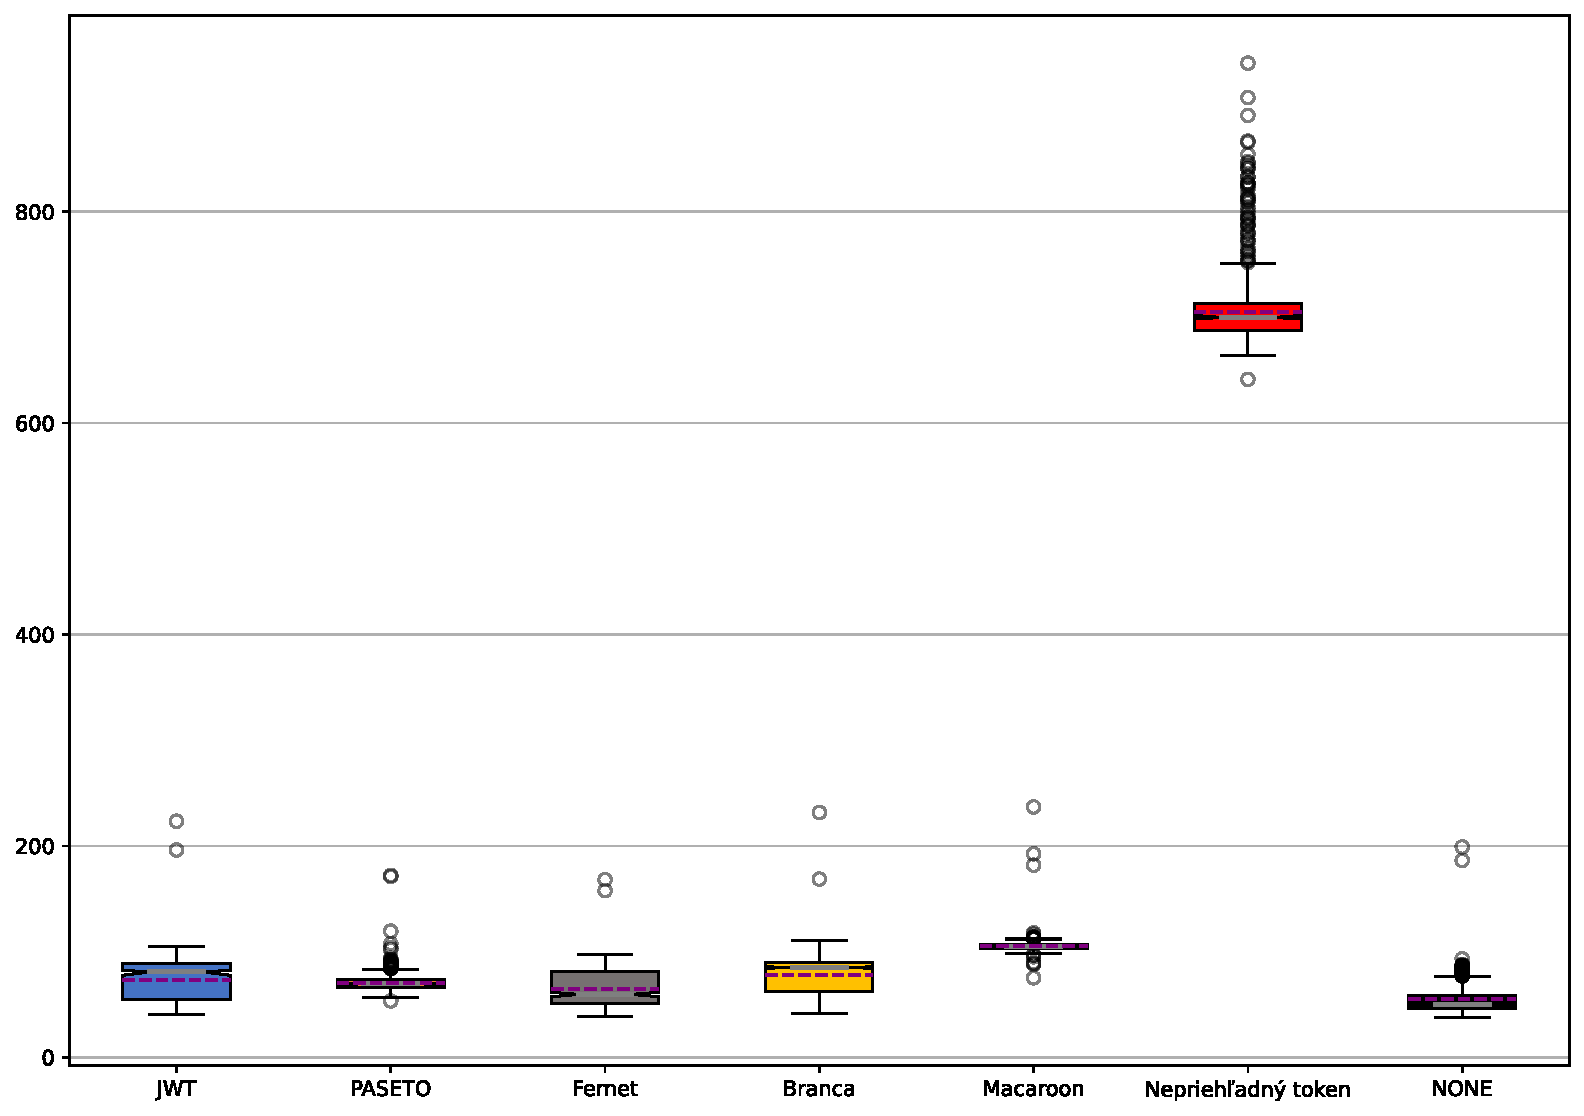
\includegraphics[width=0.7\textwidth]{images/request_boxplot_allW}}
  %popis obrazku
  \caption[Krabicový graf -- validácia, všetky hodnoty]{Krabicový graf zobrazujúci všetky namerané hodnoty pri validovaní tokenu}
  %id obrazku, pomocou ktoreho sa budeme na obrazok odvolavat
  \label{fig:request_boxplot_allW}
\end{figure}

Na grafoch \ref{fig:signin_boxplot_allW} a \ref{fig:request_boxplot_allW} sú zobrazené všetky namerané hodnoty. Všimnime si množstvo odľahlých hodnôt, čo znamená, že namerané dáta obsahovali veľa extrémnych hodnôt. Výskyt extrémnych hodnôt viac popíšeme neskôr pomocou čiarových grafov a histogramov. Taktiež si všimnime, že nepriehľadný token je výrazne pomalší ako ostatné tokeny. Toto je spôsobené tým, že rozhranie si pri generovaní nového tokenu musí tento token uložiť do databázy spolu s autorizačnými údajmi a pri validácii musí token spolu s údajmi vyhľadať v databáze. 

\begin{figure}[H]
  %vlozenie samotneho obrazku vycentrovaneho a vhodnej velkosti
  %obrazok je v subore images/session.png
  \centerline{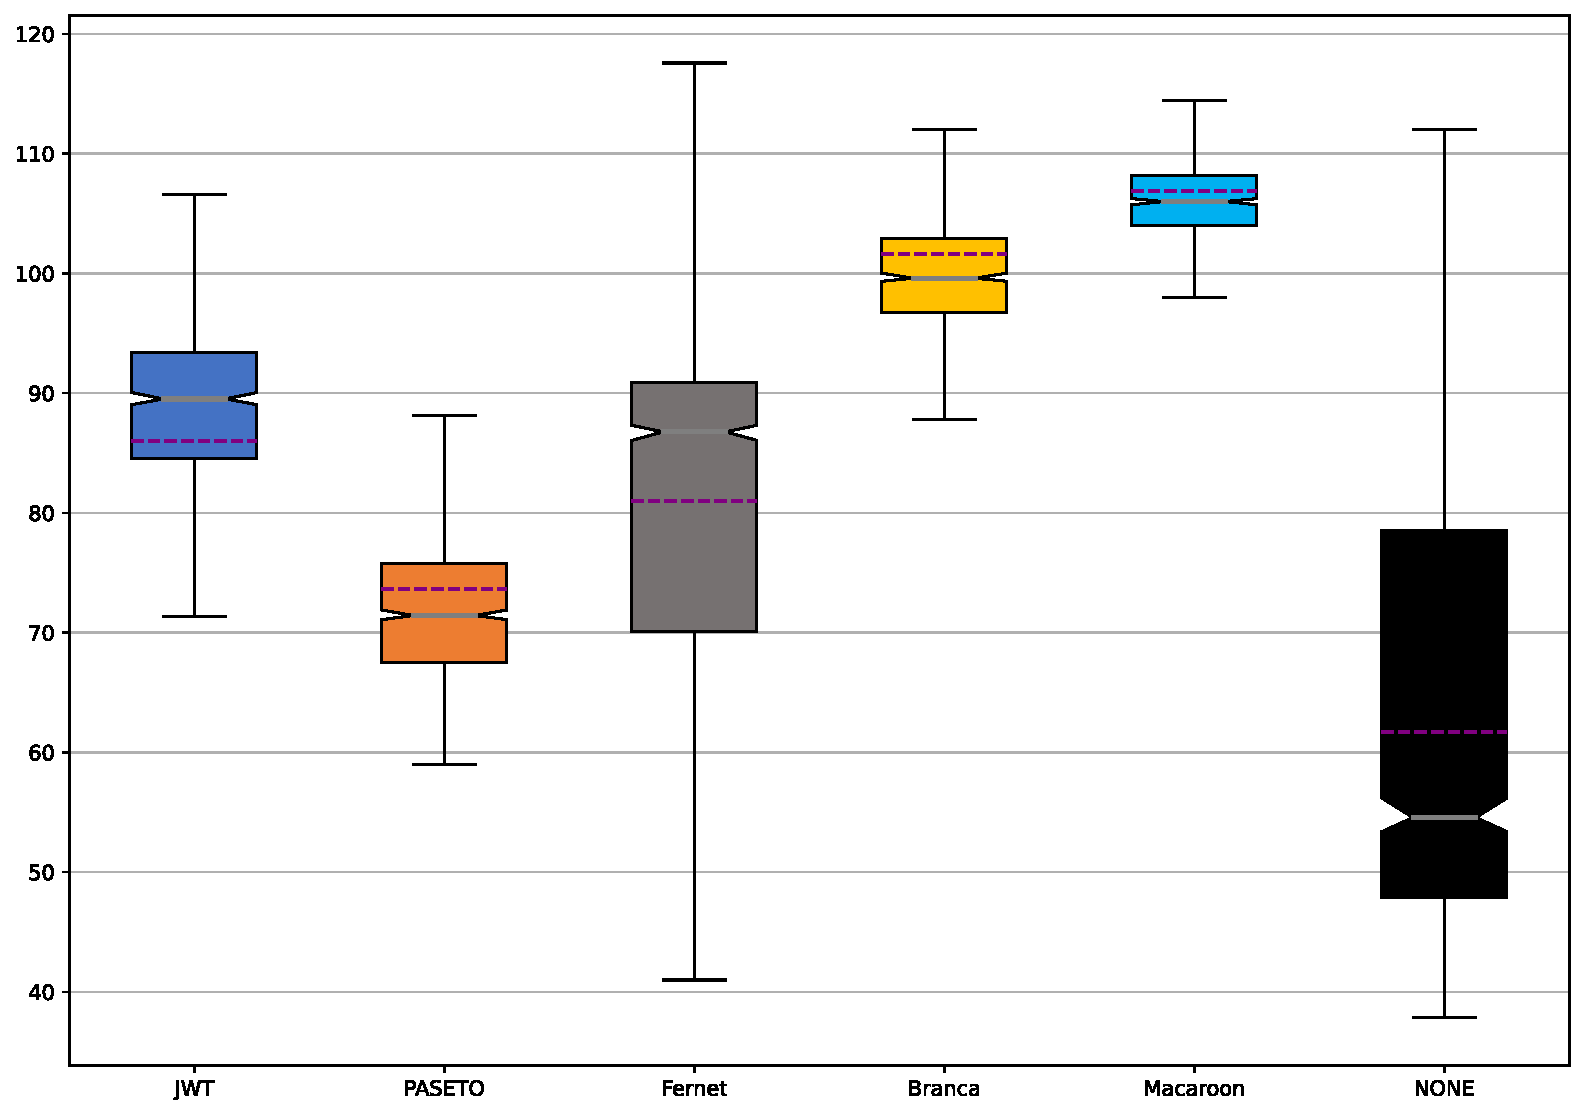
\includegraphics[width=0.7\textwidth]{images/signin_boxplot_without_opaque}}
  %popis obrazku
  \caption[Krabicový graf -- generovanie, hodnoty bez nepriehľadného tokenu]{Krabicový graf zobrazujúci namerané hodnoty bez nepriehľadného tokenu pri generovaní tokenu}
  %id obrazku, pomocou ktoreho sa budeme na obrazok odvolavat
  \label{fig:signin_boxplot_without_opaque}
\end{figure}

\begin{figure}[H]
  %vlozenie samotneho obrazku vycentrovaneho a vhodnej velkosti
  %obrazok je v subore images/session.png
  \centerline{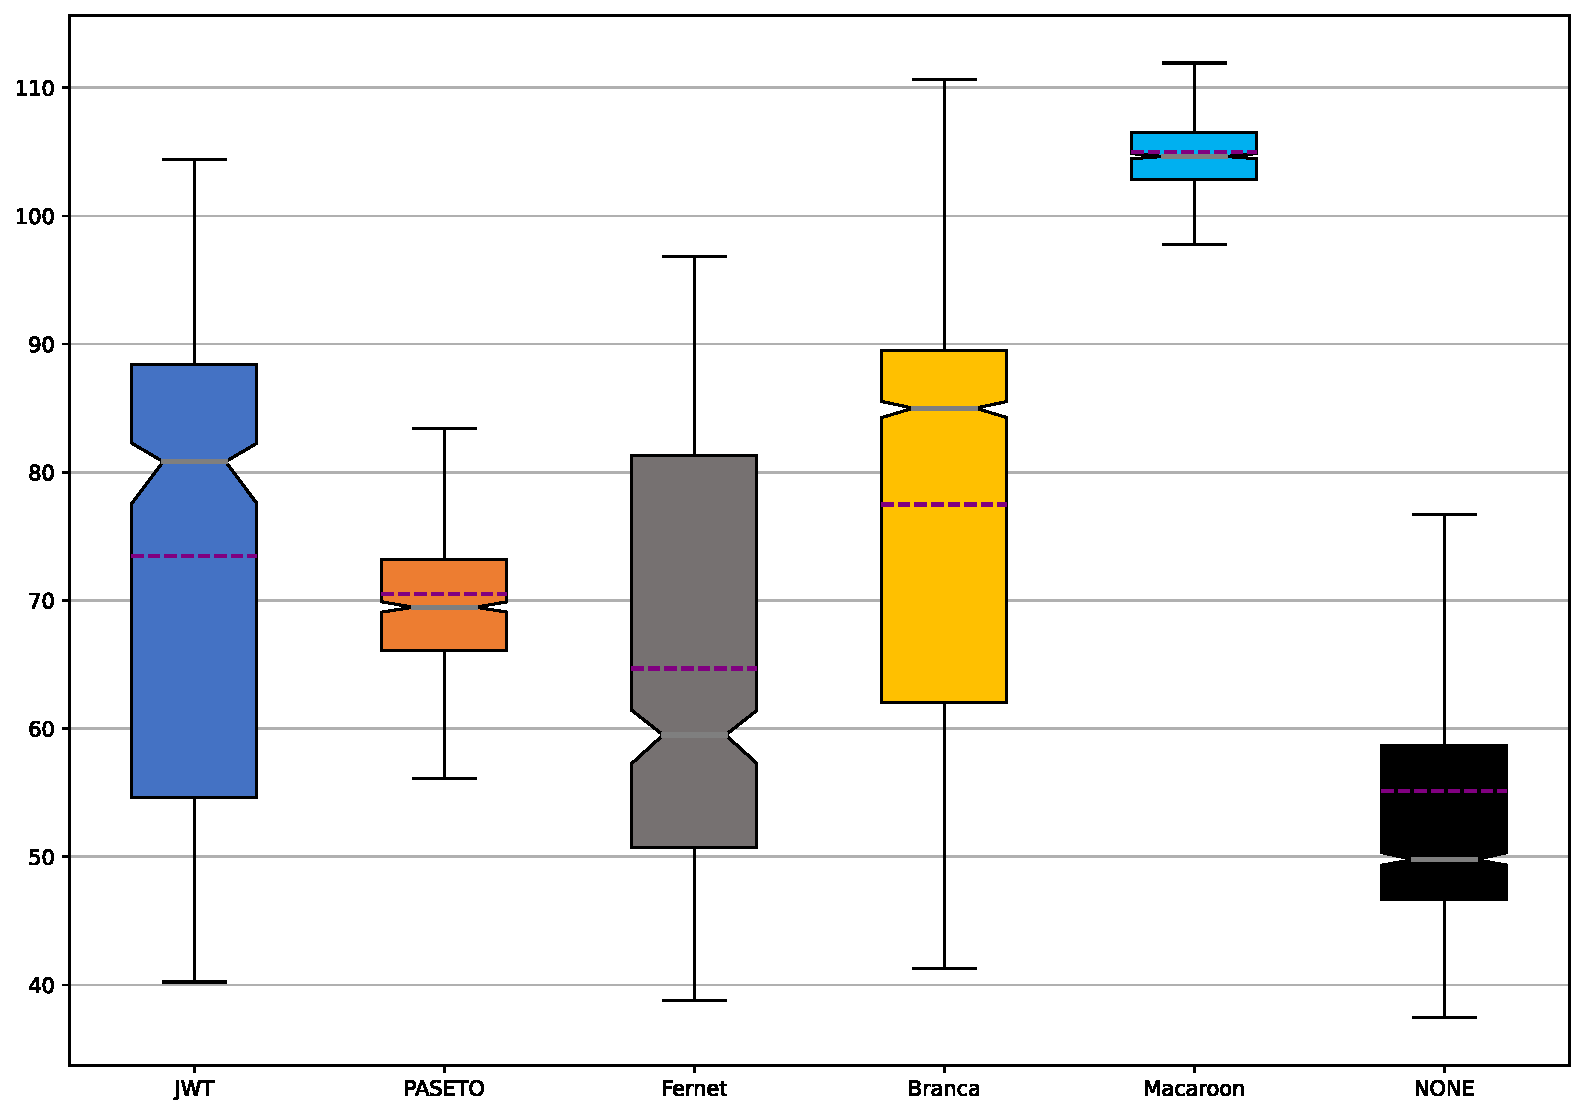
\includegraphics[width=0.7\textwidth]{images/request_boxplot_without_opaque}}
  %popis obrazku
  \caption[Krabicový graf -- validácia, hodnoty bez nepriehľadného tokenu]{Krabicový graf zobrazujúci namerané hodnoty bez nepriehľadného tokenu pri validovaní tokenu}
  %id obrazku, pomocou ktoreho sa budeme na obrazok odvolavat
  \label{fig:request_boxplot_without_opaque}
\end{figure}

Pomalosť nepriehľadného tokenu spôsobuje značnú neprehľadnosť grafov. Preto sme sa rozhodli zobraziť tokeny bez nepriehľadného tokenu. A taktiež bez odľahlých hodnôt, aby sme získali prehľadnejšie zobrazenie neextrémnych hodnôt. Tieto grafy sú zobrazené na obrázkoch \ref{fig:signin_boxplot_without_opaque} a \ref{fig:request_boxplot_without_opaque}.

Pri všetkých tokenoch vidíme zrýchlenie medzi generovaním a validáciou. Toto môže byť spôsobené tým, že veľa hodnôt používaných pri validácii aj generovaní si počítač odložil do medzipamäte (angl. cache) a pri validácií ich mal potom rýchlejšie k dispozícii. Najmenej výrazné zrýchlenie je pri Macaroons. To je pravdepodobne spôsobené tým, že Macaroons počíta viacero hodnôt pri generovaní aj validácii a taktiež má zložitú štruktúru, do ktorej sa hodnoty ukladajú. Teda manipulácia s nimi je ťažšie predvídateľná pre procesor.

\begin{figure}[H]
  %vlozenie samotneho obrazku vycentrovaneho a vhodnej velkosti
  %obrazok je v subore images/session.png
  \centerline{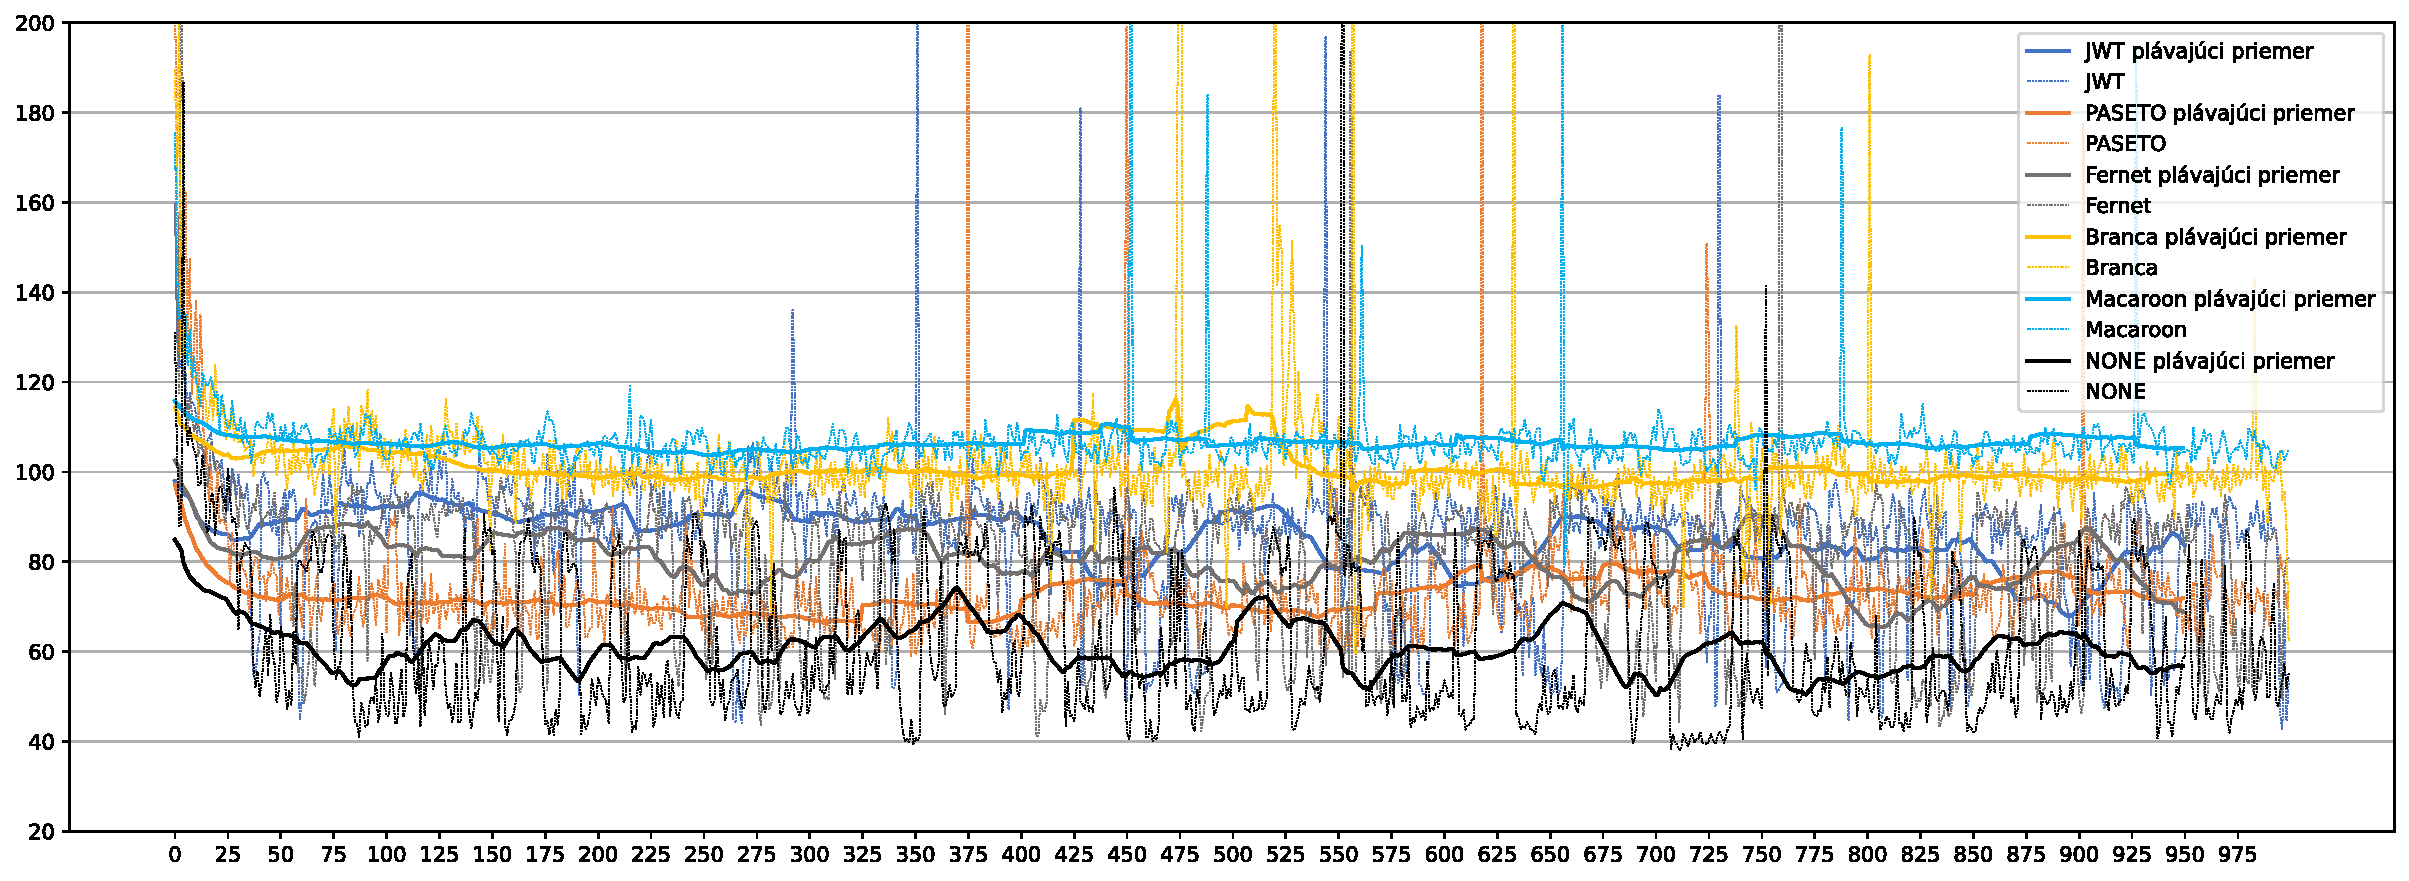
\includegraphics[width=1\textwidth]{images/signin_line_without_opaque}}
  %popis obrazku
  \caption[Čiarový graf -- generovanie, hodnoty bez nepriehľadného tokenu]{Čiarový graf zobrazujúci namerané hodnoty bez nepriehľadného tokenu pri generovaní tokenu}
  %id obrazku, pomocou ktoreho sa budeme na obrazok odvolavat
  \label{fig:signin_line_without_opaque}
\end{figure}

\begin{figure}[H]
  %vlozenie samotneho obrazku vycentrovaneho a vhodnej velkosti
  %obrazok je v subore images/session.png
  \centerline{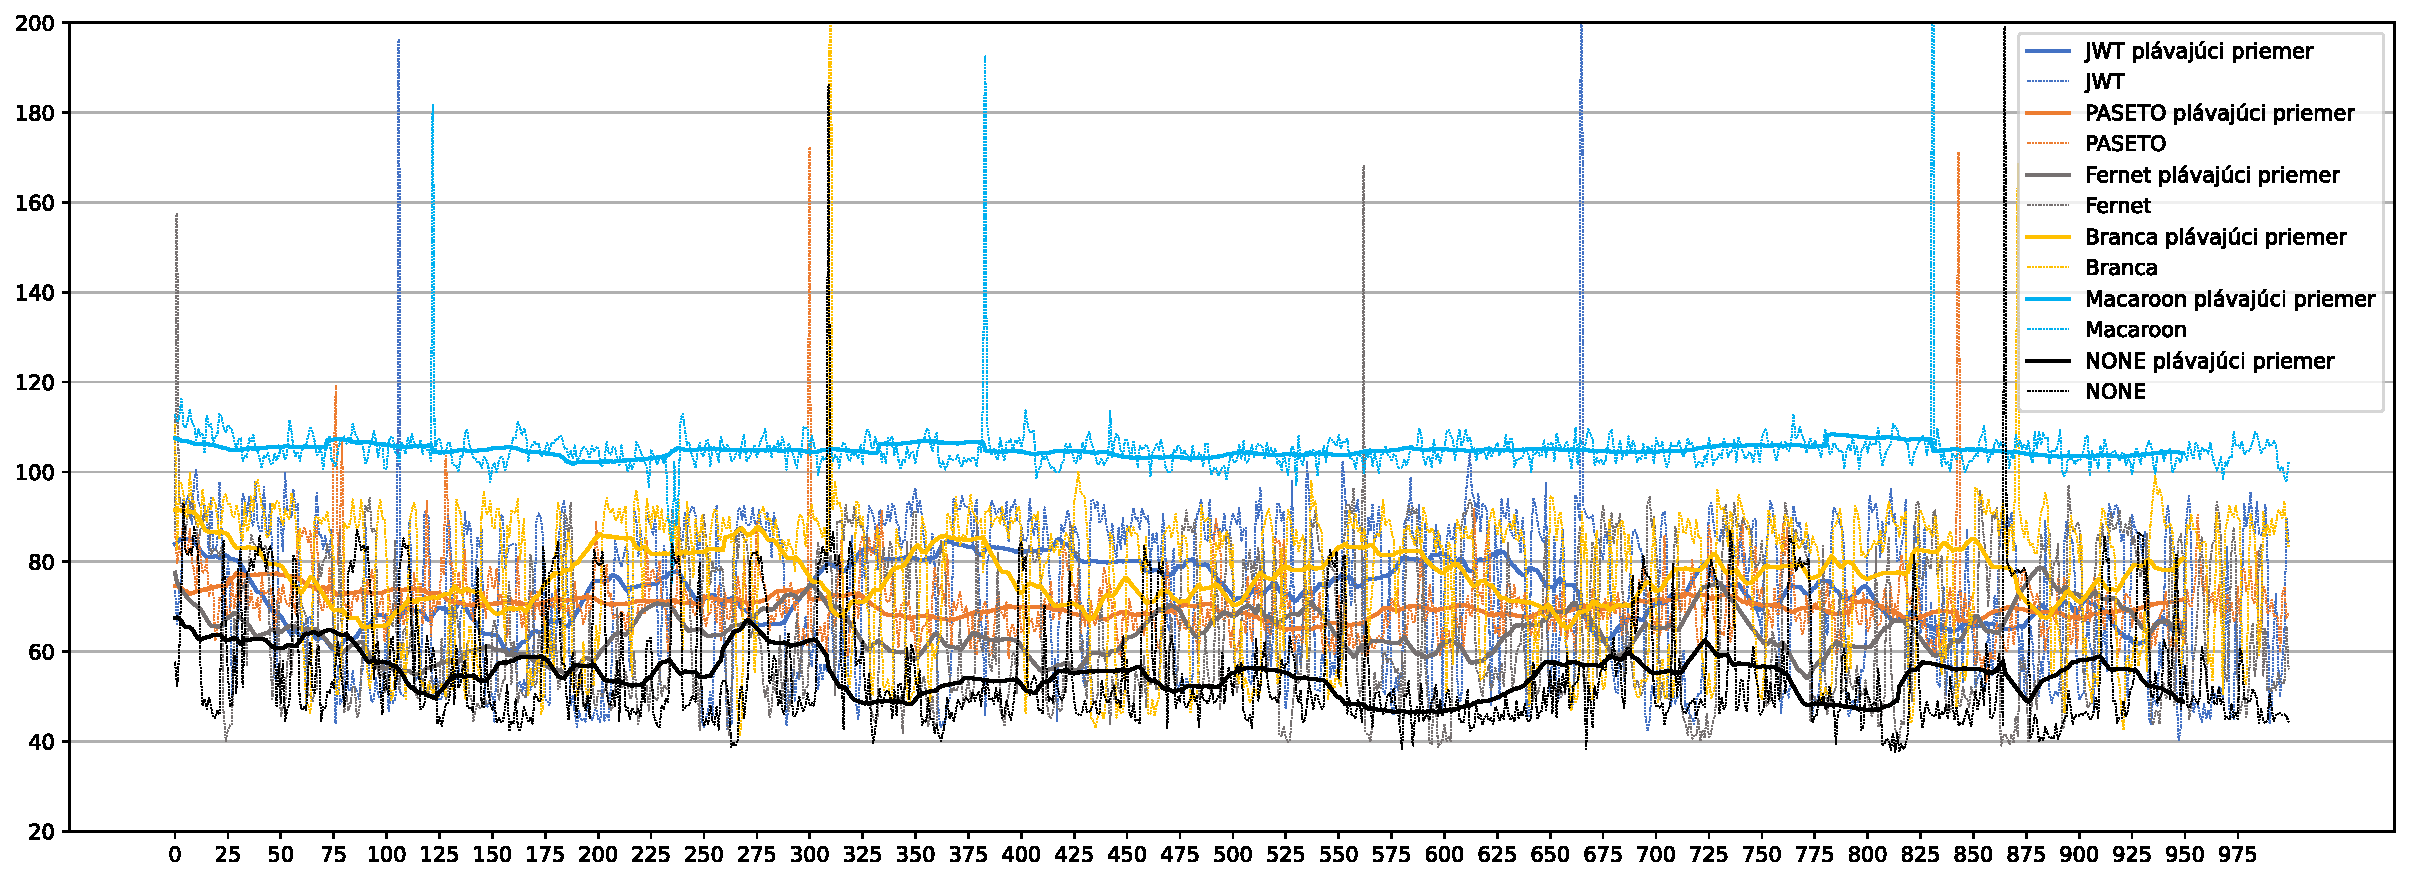
\includegraphics[width=1\textwidth]{images/request_line_without_opaque}}
  %popis obrazku
  \caption[Čiarový graf -- validácia, hodnoty bez nepriehľadného tokenu]{Čiarový graf zobrazujúci namerané hodnoty bez nepriehľadného tokenu pri validovaní tokenu}
  %id obrazku, pomocou ktoreho sa budeme na obrazok odvolavat
  \label{fig:request_line_without_opaque}
\end{figure}

Na priamu vizualizáciu všetkých nameraných dát sme použili čiarový graf. Na ľavej osi je rýchlosť v milisekundách a na dolnej osi je poradové číslo merania. Pre vyššiu prehľadnosť grafu sme vypočítali a zobrali aj plávajúci priemer hodnôt. Plávajúci priemer je vypočítaný ako priemer 50 konsekutívnych hodnôt. Tento priemer je na grafe zobrazený plnou čiarou a všetky hodnoty sú zobrazené bodkovanými čiarami. Ako sme si všimli už pri krabicovom grafe, rýchlosť nepriehľadného tokenu je výrazne menšia ako rýchlosť ostatných tokenov. Preto sme sa rozhodli zobraziť graf bez nepriehľadného tokenu. Popísané čiarové grafy sú zobrazené na obrázkoch \ref{fig:signin_line_without_opaque} a \ref{fig:request_line_without_opaque}.


Vidíme, že namerané hodnoty výrazne skáču, čo dokazujú aj histogramy na obrázkoch \ref{fig:signin_histogram_all} a \ref{fig:request_histogram_all}. Histogramy majú na ľavej osi počet meraní a na dolnej osi rýchlosť v milisekundách. Toto správanie môžeme vysvetliť tým, že rozhranie aj klienta sme spúšťali na jednom počítači, na ktorom samozrejme bežali aj iné procesy. Výkyvy v nameraných hodnotách sú teda pravdepodobne spôsobené prepínaním procesov a prideľovaním zdrojov na počítači. Až na niektoré extrémne odchýlky sú výkyvy v rámci všetkých tokenov podobné. Najmä na čiarovom grafe zobrazujúcom generovanie tokenu vidíme, že namerané hodnoty v prvých približne 50 meraniach sú vyššie ako v ostatných meraniach a postupne klesajú. Toto sa dá vysvetliť online kompiláciou, už za behu, často používaného kódu. Táto interpretácia sedí aj s tým, že pri validácii tokenu sa tento jav nevyskytuje. Validácia sa totiž meria až po zmeraní generovania tokenu a v rámci jedného spustenia kódu rozhrania aj klienta. Kódy rozhrania aj klienta sú už teda dokompilované.


Pre číselné porovnanie rýchlosti tokenov sme z čiarových grafov \ref{fig:signin_line_without_opaque} a \ref{fig:request_line_without_opaque} odstránili bodkované čiary a nechali len plné čiary, reprezentujúce plávajúce priemery. Od hodnôt tokenov sme odpočítali hodnoty namerané s NONE tokenom, aby sme porovnávali čisto rýchlosť generovania a validácie tokenov bez réžie okolo spracovania požiadaviek. Tieto grafy sú zobrazené na obrázkoch \ref{fig:signin_line_minus_none_without_opaque} a \ref{fig:request_line_minus_none_without_opaque}.

\begin{figure}[H]
  %vlozenie samotneho obrazku vycentrovaneho a vhodnej velkosti
  %obrazok je v subore images/session.png
  \centerline{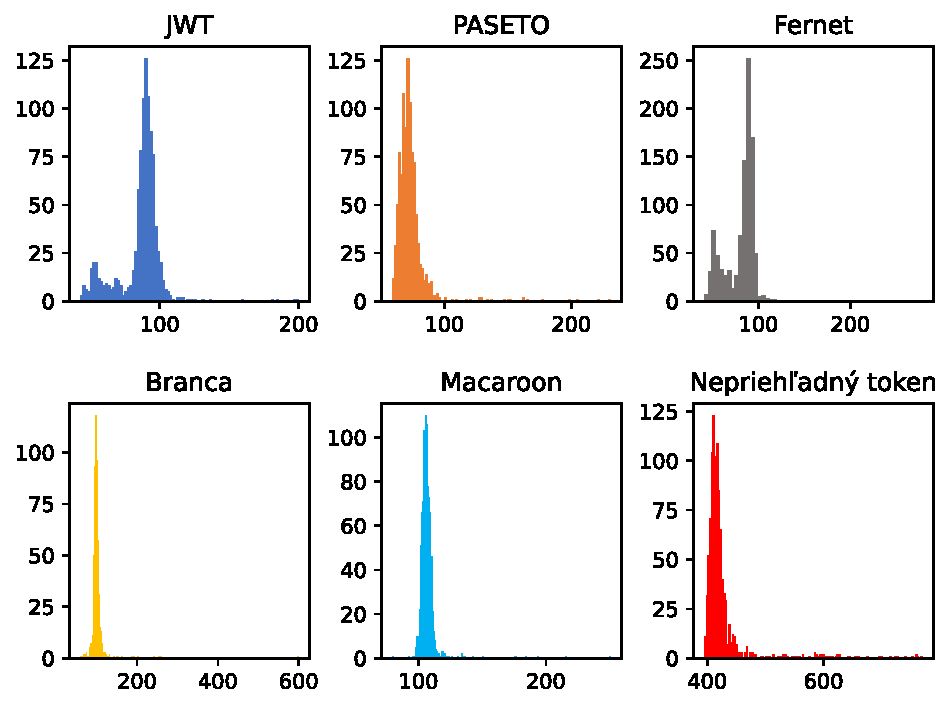
\includegraphics[width=0.7\textwidth]{images/signin_histogram_all}}
  %popis obrazku
  \caption[Histogram -- generovanie, všetky hodnoty]{Histogram zobrazujúci všetky namerané hodnoty pri generovaní tokenu}
  %id obrazku, pomocou ktoreho sa budeme na obrazok odvolavat
  \label{fig:signin_histogram_all}
\end{figure}

\begin{figure}[H]
  %vlozenie samotneho obrazku vycentrovaneho a vhodnej velkosti
  %obrazok je v subore images/session.png
  \centerline{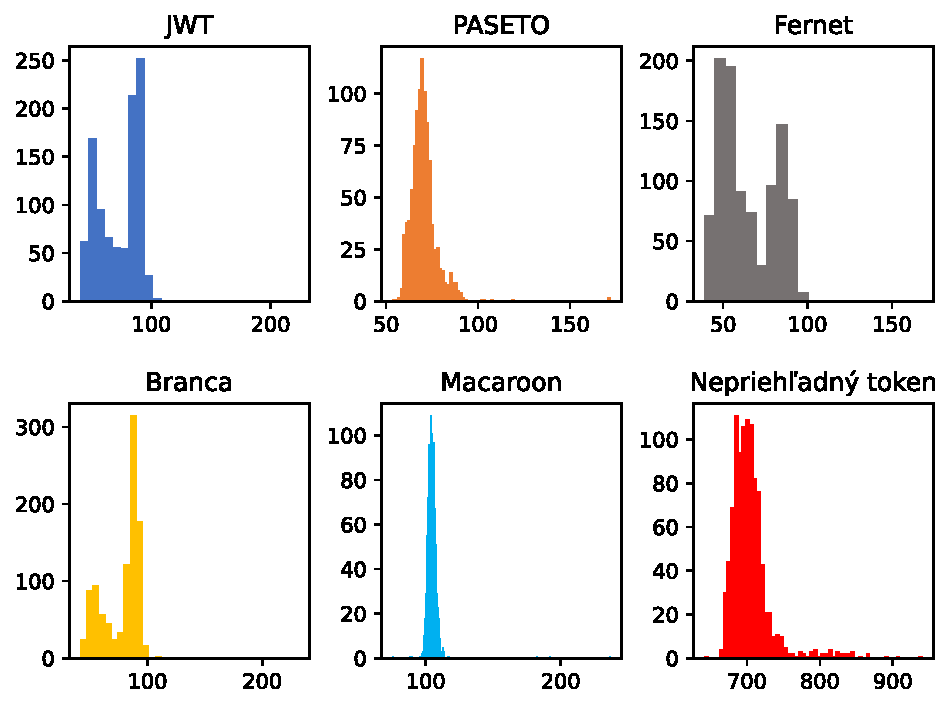
\includegraphics[width=0.7\textwidth]{images/request_histogram_all}}
  %popis obrazku
  \caption[Histogram -- validácia, všetky hodnoty]{Histogram zobrazujúci všetky namerané hodnoty pri validovaní tokenu}
  %id obrazku, pomocou ktoreho sa budeme na obrazok odvolavat
  \label{fig:request_histogram_all}
\end{figure}

Aj hodnoty plávajúcich priemerov nie sú úplne rovnomerné a nedá sa z nich priamo porovnať rýchlosť tokenov. Preto sme sa rozhodli porovnať rýchlosť na základe aritmetického priemeru všetkých nameraných hodnôt (tiež po odpočítaní NONE tokenu). Toto porovnanie je zobrazené v grafoch \ref{fig:signin_line_avg_without_opaque} a \ref{fig:request_line_avg_without_opaque}. Graf má odrezanú ľavú os tak, aby nezobrazoval nepriehľadný token. V takomto prípade sú prehľadnejšie vidieť rozdiely medzi ostatnými tokenmi. V legendách je zobrazený aritmetický priemer všetkých nameraných hodnôt. V legende je uvedený aj aritmetický priemer rýchlosti nepriehľadného tokenu.

\begin{figure}[H]
  %vlozenie samotneho obrazku vycentrovaneho a vhodnej velkosti
  %obrazok je v subore images/session.png
  \centerline{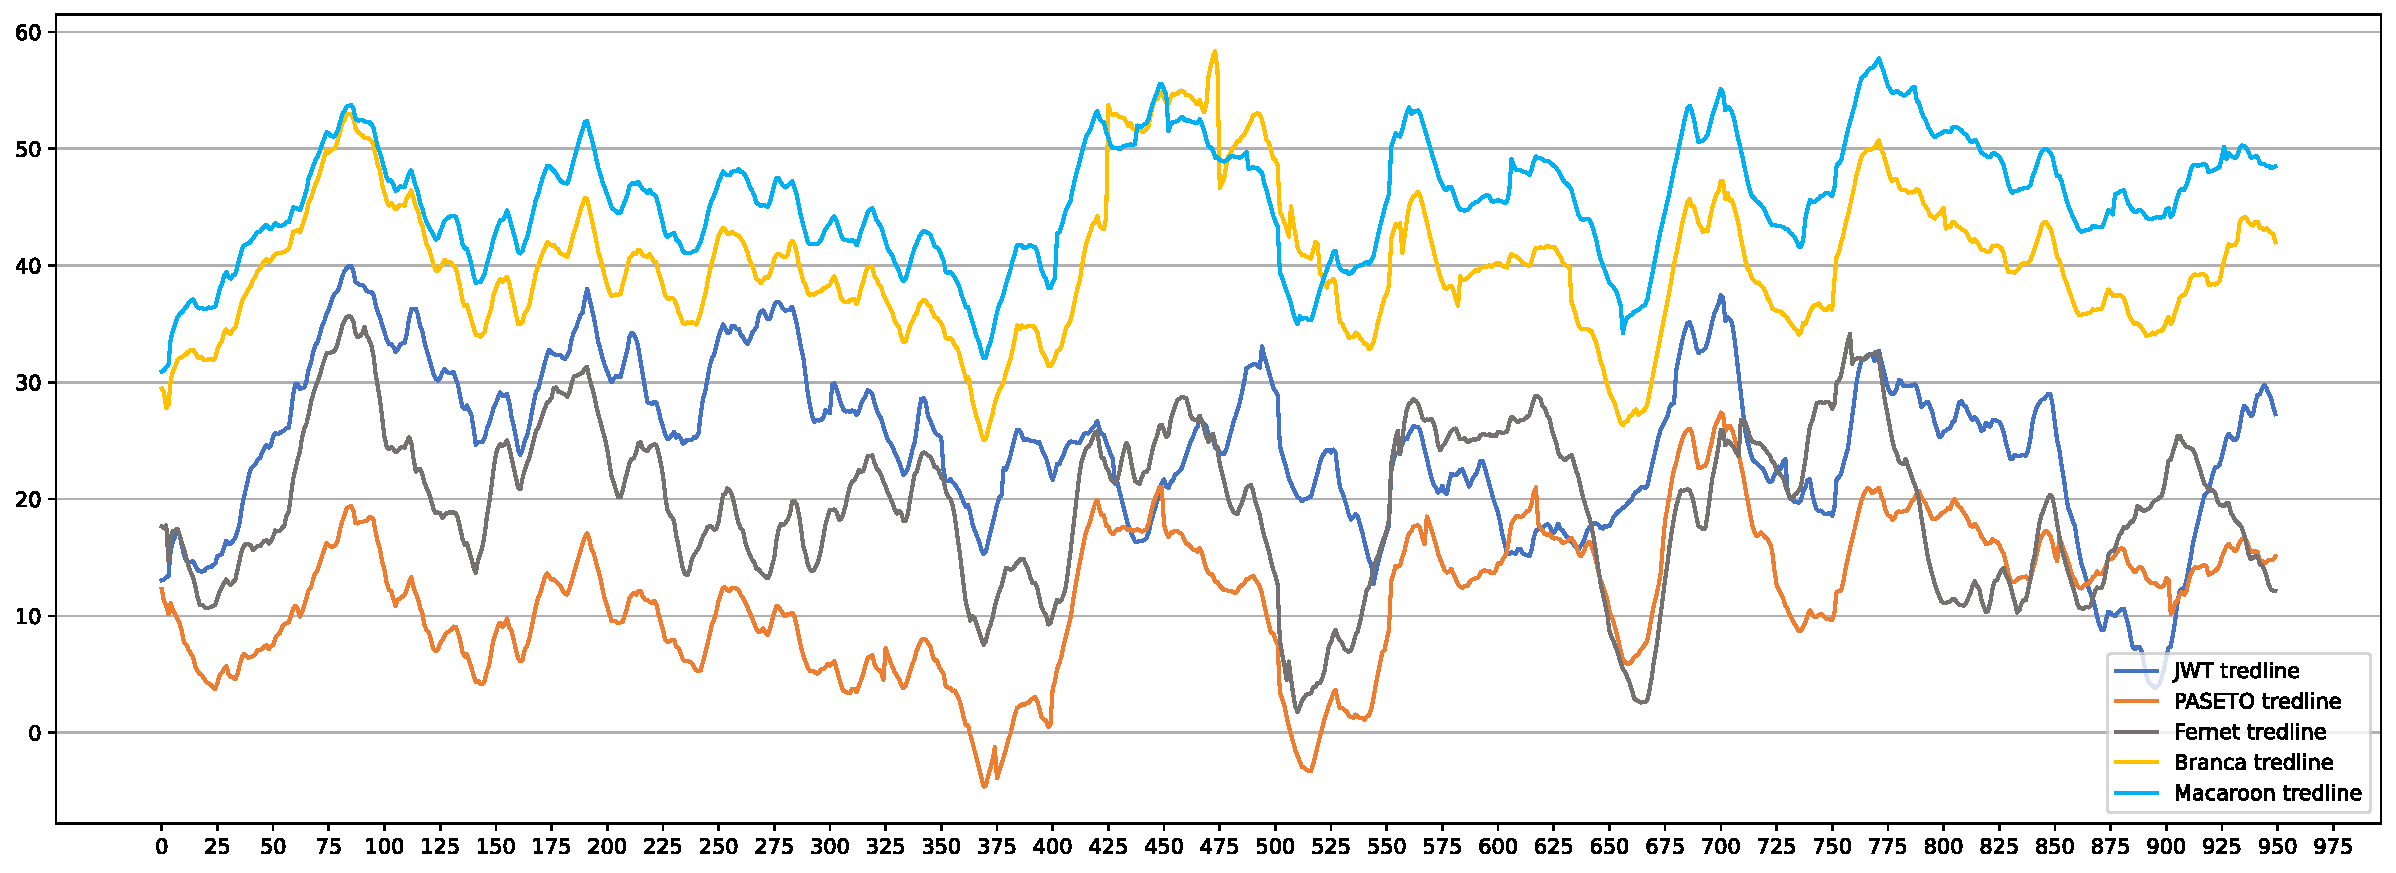
\includegraphics[width=1\textwidth]{images/signin_line_minus_none_without_opaque}}
  %popis obrazku
  \caption[Čiarový graf -- generovanie, odpočítaný NONE token]{Čiarový graf zobrazujúci namerané hodnoty s odpočítaným NONE tokenom bez nepriehľadného tokenu pri generovaní tokenu}
  %id obrazku, pomocou ktoreho sa budeme na obrazok odvolavat
  \label{fig:signin_line_minus_none_without_opaque}
\end{figure}

\begin{figure}[H]
  %vlozenie samotneho obrazku vycentrovaneho a vhodnej velkosti
  %obrazok je v subore images/session.png
  \centerline{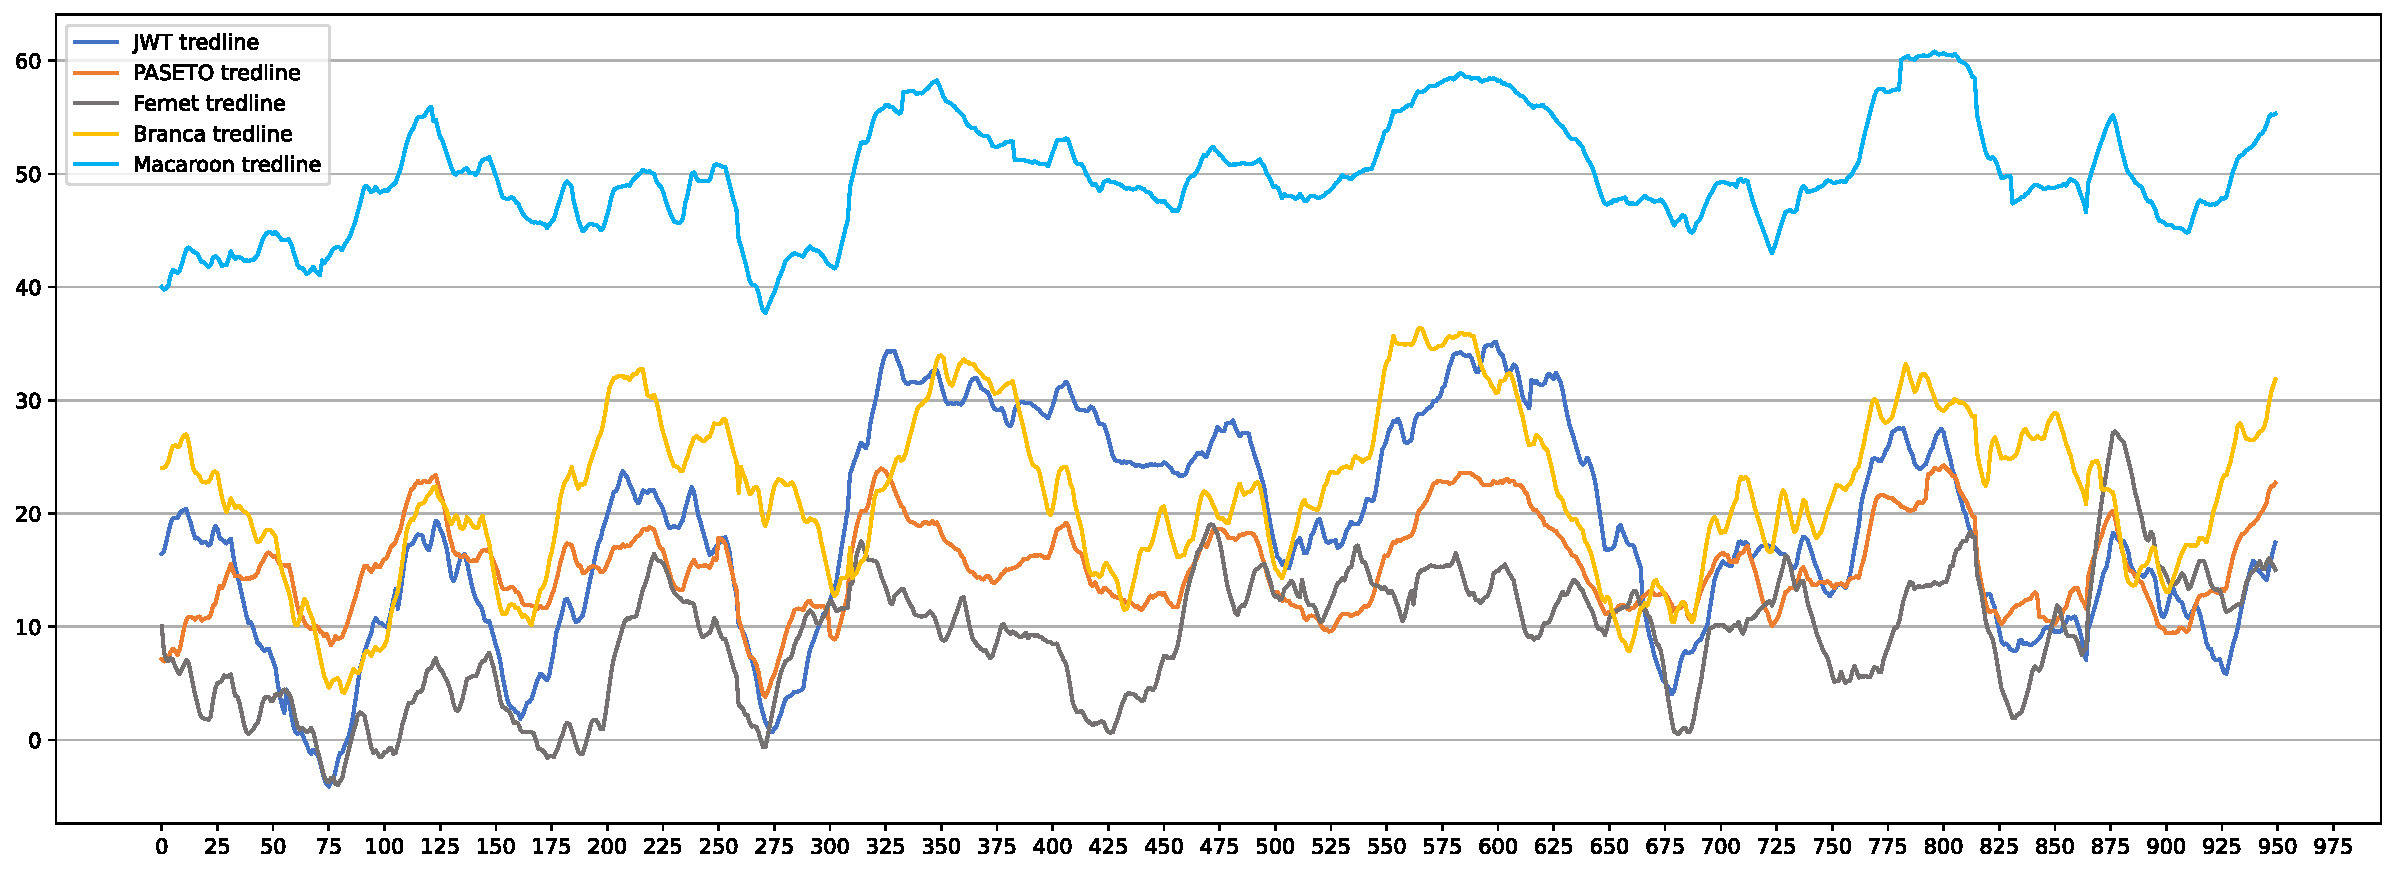
\includegraphics[width=1\textwidth]{images/request_line_minus_none_without_opaque}}
  %popis obrazku
  \caption[Čiarový graf -- validácia, odpočítaný NONE token]{Čiarový graf zobrazujúci namerané hodnoty s odpočítaným NONE tokenom bez nepriehľadného tokenu pri validovaní tokenu}
  %id obrazku, pomocou ktoreho sa budeme na obrazok odvolavat
  \label{fig:request_line_minus_none_without_opaque}
\end{figure}


\begin{figure}[H]
  %vlozenie samotneho obrazku vycentrovaneho a vhodnej velkosti
  %obrazok je v subore images/session.png
  \centerline{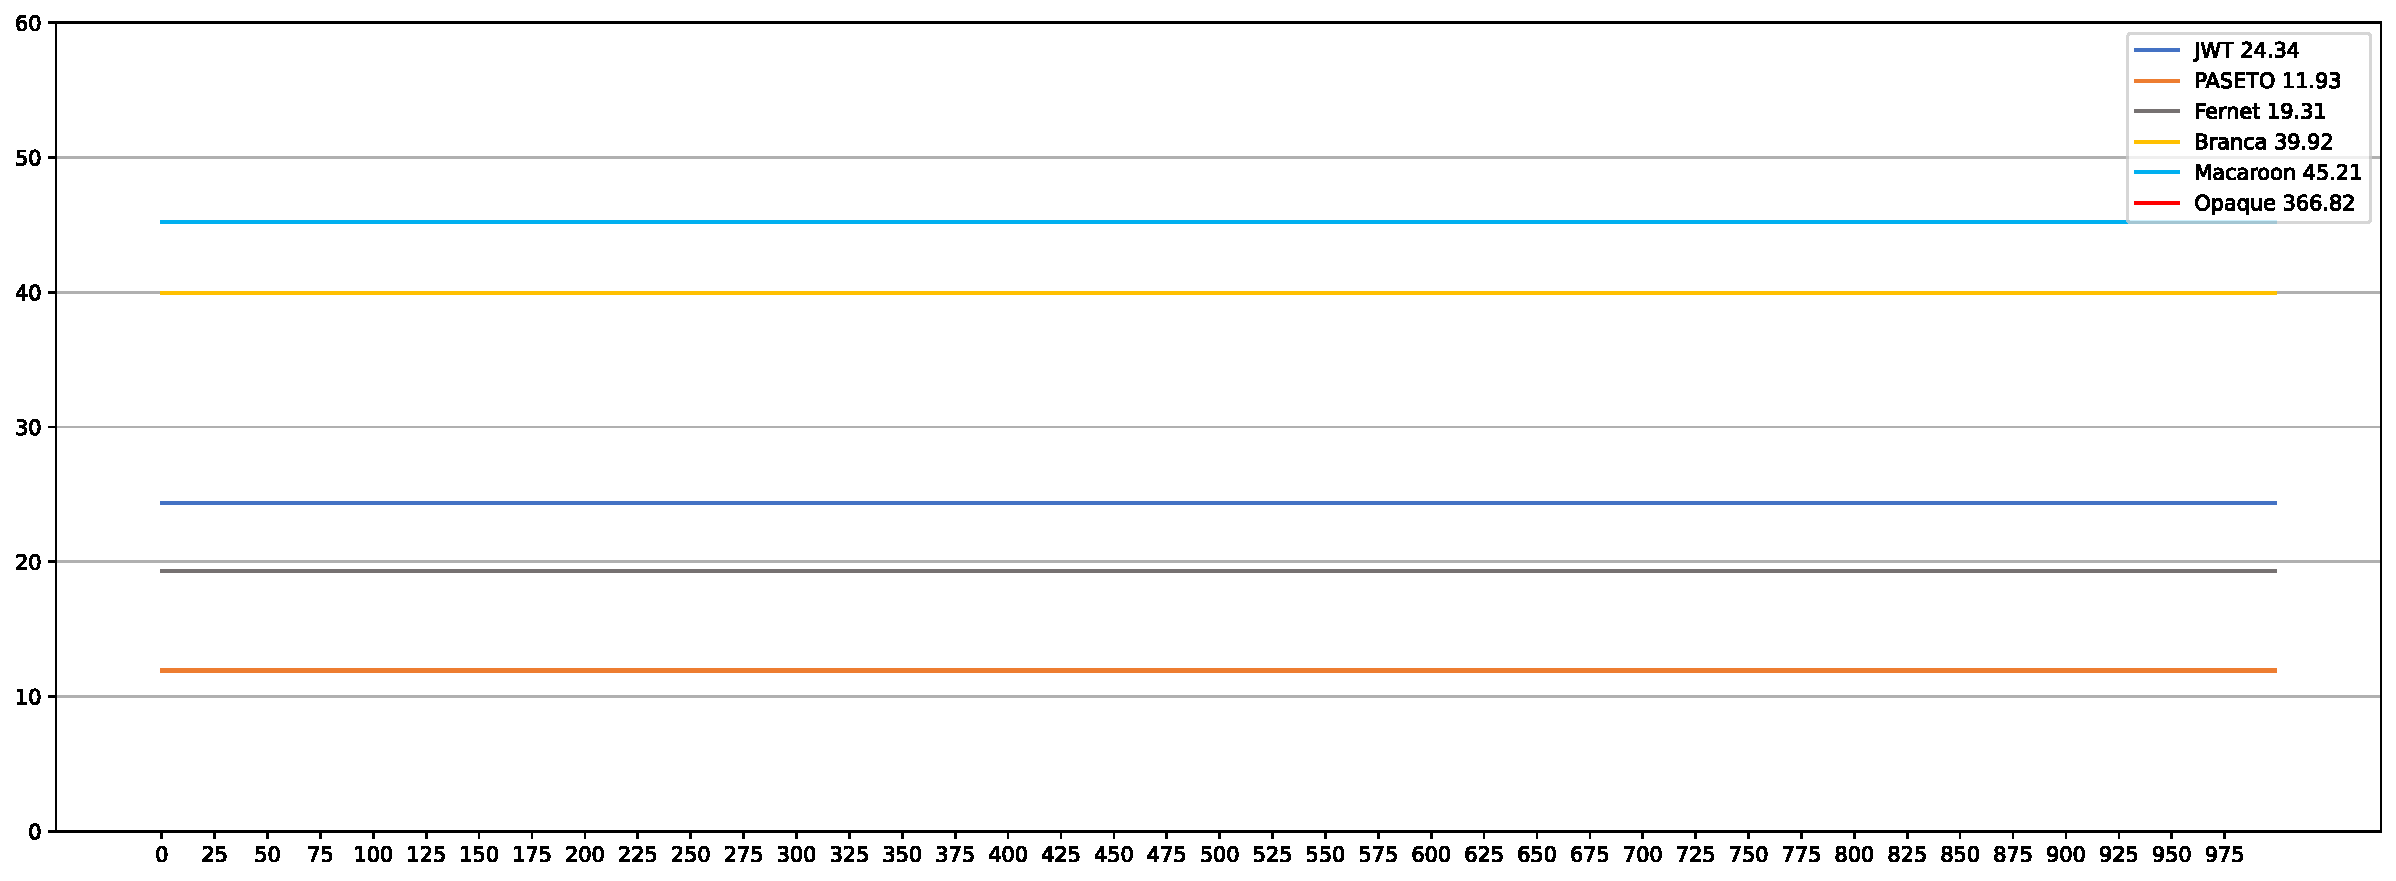
\includegraphics[width=1\textwidth]{images/signin_line_avg_without_opaque}}
  %popis obrazku
  \caption[Čiarový graf -- generovanie, konštantný priemer]{Čiarový graf zobrazujúci aritmetický priemer nameraných hodnôt s odpočítaným NONE tokenom bez nepriehľadného tokenu pri generovaní tokenu}
  %id obrazku, pomocou ktoreho sa budeme na obrazok odvolavat
  \label{fig:signin_line_avg_without_opaque}
\end{figure}

\begin{figure}[H]
  %vlozenie samotneho obrazku vycentrovaneho a vhodnej velkosti
  %obrazok je v subore images/session.png
  \centerline{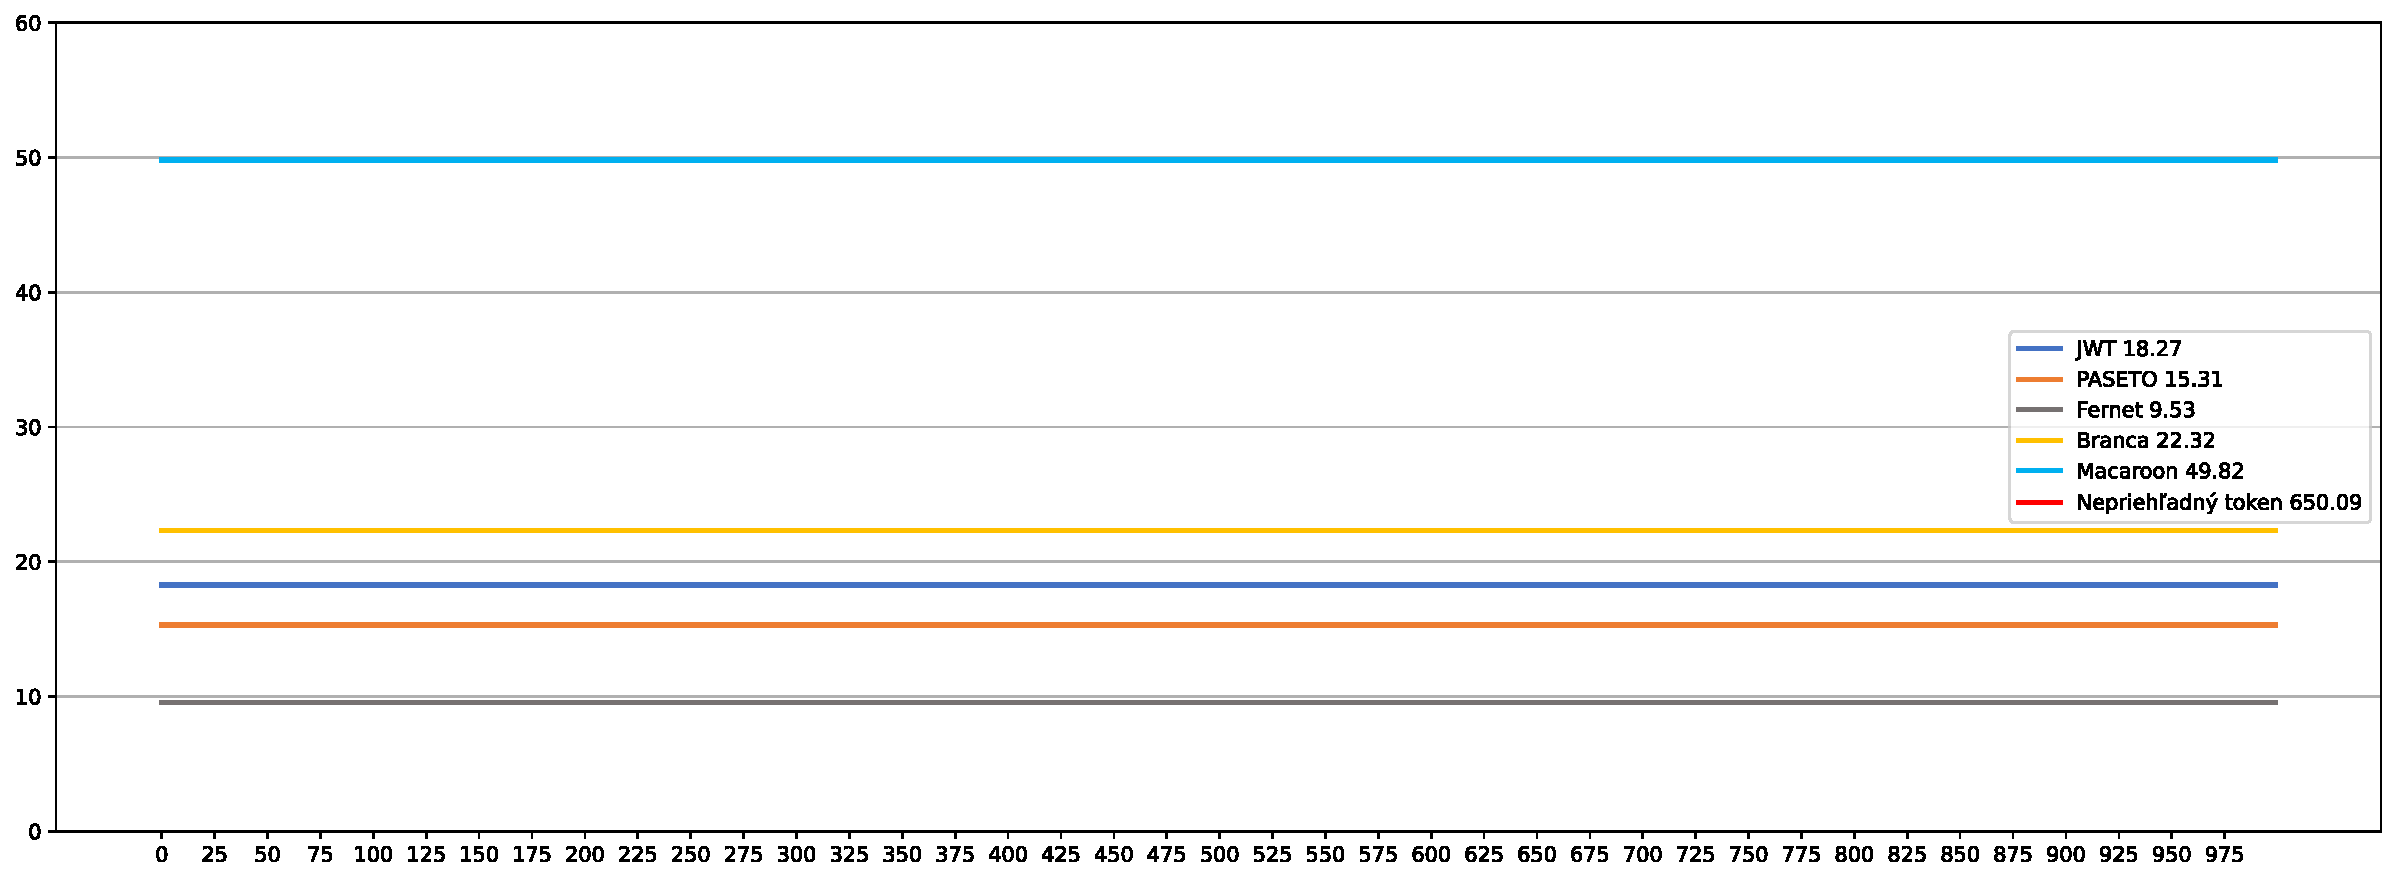
\includegraphics[width=1\textwidth]{images/request_line_avg_without_opaque}}
  %popis obrazku
  \caption[Čiarový graf -- validácia, konštantný priemer]{Čiarový graf zobrazujúci aritmetický priemer nameraných hodnôt s odpočítaným NONE tokenom bez nepriehľadného tokenu pri validovaní tokenu}
  %id obrazku, pomocou ktoreho sa budeme na obrazok odvolavat
  \label{fig:request_line_avg_without_opaque}
\end{figure}

Ako sme spomenuli už vyššie, nepriehľadný token je pre využívanie databázy výrazne pomalší ako ostatné tokeny. Konkrétne je v priemere v prípade generovania 8-30 krát pomalší a v prípade validácie 13-68 krát pomalší.

Prekvapivým výsledkom je, že Macaroons je okrem nepriehľadného tokenu najpomalší pri generovaní aj validácii, pretože okrem nepriehľadného tokenu ide o jediný token, ktorého telo sa nešifruje. Tento výsledok je možné vysvetliť tým, že Macaroons je najkomplexnejší token, formátom aj procesom generovania. Pri generovaní sa aplikuje podpisová funkcia raz pri vytvorení nového tokenu a následne toľko krát koľko pravidiel do tokenu pridávame, v~našom prípade štyrikrát. Podobne pri validácii tokenu sa musí vypočítať podpis tokenu postupnou aplikáciou podpisovej funkcie na každé pravidlo v tele tokenu. Macaroons bol vytvorený pre komplexné systémy pre jeho flexibilitu spočívajúcu v možnosti pridávať pravidlá ľubovoľnou entitou a elegantného riešenia zapojenia tretích strán do autorizácie pomocou pravidiel tretích strán. Preto je pre jednoduchý systém, ako je nami implementované rozhranie, Macaroons nevhodný.

Zaujímavým pozorovaním je výrazné zrýchlenie validácie nepriehľadného tokenu a Branca tokenu oproti jeho generovaniu. Vyššie sme odôvodnili prečo pri všetkých tokenoch vidíme zrýchlenie validácie oproti generovaniu. V prípade týchto tokenov je ale zrýchlenie najvýraznejšie. V oboch prípadoch je takmer dvojnásobné. Rozhranie využíva jednoduchú súborovú databázu sqlite. Pri generovaní nepriehľadného tokenu sa teda pravdepodobne databáza načíta do operačnej pamäti z disku a ďalej pri validácii sa už číta iba z operačnej pamäte, ktorá je výrazne rýchlejšia.

Pri Branca tokene predpokladáme, že ide o rozdiel rýchlosti šifrovacej funkcie pri šifrovaní a dešifrovaní. Táto funkcie je totiž odlišná od funkcií použitých v ostatných tokenoch.

Celkovo najrýchlejší je pri generovaní PASETO, konkrétne 1,6-3,8 krát rýchlejší. Pri validácii je najrýchlejší Fernet, konkrétne 1,6-5,2 krát rýchlejší. V oboch prípadoch porovnávame najrýchlejší token s ostatnými tokenmi okrem nepriehľadného tokenu. Uvedomme si však, že najmä v prípade validácie sú rozdiely medzi JWT, PASETO, Fernet a Branca takmer zanedbateľné. Rozdiel ich rýchlostí je najviac 12,78 ms pri súčte 100 meraní. Teda 0,13 ms na jednu požiadavku.